\subsection{Tally Sticks}


\content{
        It is often conjectured that the earliest counting methods was 'tally
        sticks'. 
}{% presentation
\vspace{2in}
}{% nopresentation
\vspace{2in}
}{% comments
This uses the idea of what we now call a one-to-one coorespondence. \\
It is clear that this system is insufficient for most purposes. 
}

\subsubsection{The Inca Civilization}

\content{
    The Inca do not seem to have had a complicated counting system, which seems
    to be centered on record keeping. One way that they accomplished this was
    through the use of counting boards. Let's take a look.\\

    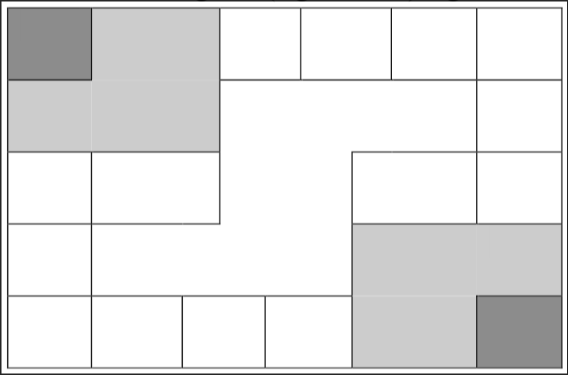
\includegraphics[scale=.25]{counting-board.png}
}{% presentation
\vspace{1in}
}{% nopresentation
\vspace{1in}
}{% comments
The outer twelve white boxes are ones\\
The two larger white boxes are twos\\
middle region is 3\\
light grey is 6\\
dark is 12
}

\content{
        Let's assume that the black pebbles represent dogs, and the gray, cats.
        How many of each is found according to the following counting board. \\

        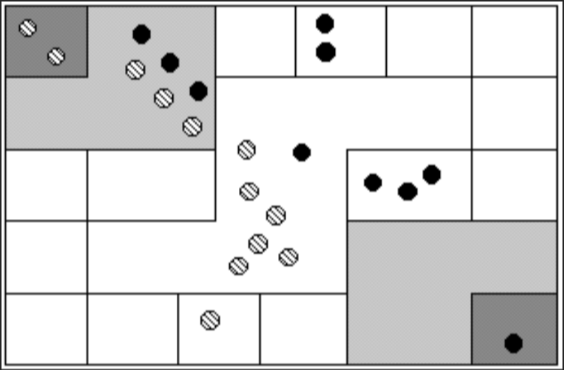
\includegraphics[scale=0.25]{counting-board-ex.png}

}{% presentation
\vspace{2in}
}{% nopresentation
\vspace{2in}
}{% comments
41 dogs
}

\content{
        The quipu was another method used for a more permanent form of counting,
        useful for keeping track of numbers over time. \\

        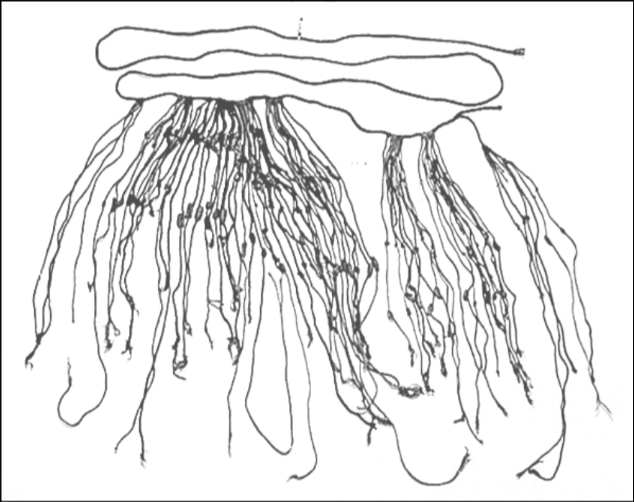
\includegraphics[scale=0.25]{quipu.png} \\

        As we can see, these can get quite complicated, and are composed of
        strings (called H strings by some researchers) attached to a main cord. 
        Counting was performed by tying a series of knots into the H strings
        according to the following: 
        \begin{itemize}
        \item A figure 8 knot on the end of a string to denote 1
        \item A multiply looped knot to denote 2-9
        \item a single knot higher up on the string to denote 10, 100, 1000, or
        10,000
        \end{itemize}
        Let's see an example. 
}{% presentation
}{% nopresentation
}{% comments
}

\content{
        \begin{example} What numbers are represented on the following quipu. \\

        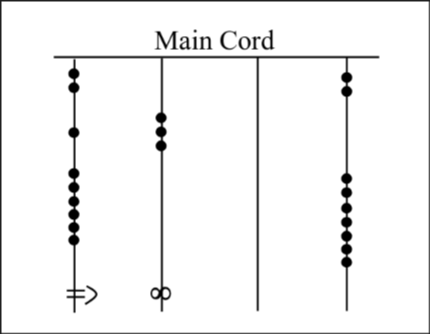
\includegraphics[scale=0.25]{quipu-ex.png}
        \end{example}
}{% presentation
}{% nopresentation
}{% comments
The figure 8 denotes a figure 8 knot, the dots represent simple knots, and the
lines with arc denote 2-9, depending on how many loops there are. 
}

\content{
        \begin{example} Take your quipu, and use it to record the date of your
        birth, using one H string for the year, another for the month, and
        another for the day. 
        \end{example}
}{% presentation
}{% nopresentation
}{% comments
Note that this takes some forethought, placing the thousands too low will make
it so in later strings you may not have enough room. 
}

\subsubsection{The Development of a System}


\content{
The Brahmi numeral system was used in various locations throughout the world for
several centuries, and consisted of symbols for many different numbers, which,
when written, were added together to find the result. A table of some of the
symbols is as follows: \\

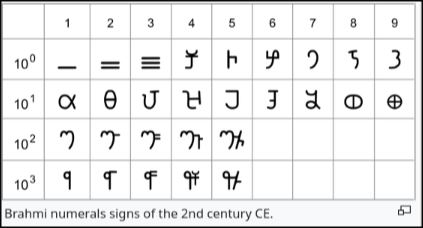
\includegraphics[scale=0.45]{brahmi-symbols.png}

Is there anything weird (to us anyway) about this number system? 
}{% presentation
\vspace{1in}
}{% nopresentation
\vspace{1in}
}{% comments
No symbol for zero! So this cannot be a positional system like the one we use
today. \\

Image taken from \\
{\tiny https://en.wikipedia.org/wiki/Brahmi\_numerals}
}


\content{
Let's take a look at how our current system developed in the textbook. 
}{% presentation
}{% nopresentation
}{% comments
}


\subsection{Positional Systems}

\content{
        As we have noticed, the notion of `position' is extremely valuable, but
        it took a long time for this idea to develop. Let's discuss some of the
        basics of what a posisitional system is. 
}{% presentation
\vspace{3in}
}{% nopresentation
\vspace{3in}
}{% comments
Write a number, explain breifly what each position is, this is pretty basic.
Note that ancient civilizations did not neccesarily use 10 as their base. 
}
